\documentclass{article}
\usepackage[utf8]{inputenc}
\usepackage[spanish,mexico]{babel}
\usepackage{array,booktabs} 
\usepackage[table]{xcolor}
\usepackage{amsmath}
\usepackage{amssymb}
\usepackage{graphicx}
\usepackage{cite}
\usepackage{color}
\usepackage{multicol}
\usepackage{ragged2e}
\usepackage{verbatim}
\usepackage[margin=2.5cm,footskip=0.25in]{geometry}
\usepackage{graphicx} % figuras
\usepackage{subfigure} % subfiguras

\oddsidemargin = 0 cm
\textwidth = 17 cm
\topmargin = -2 cm
\textheight = 26 cm  

\usepackage[spanish]{babel}



\title{Proyecto}
\usepackage[hidelinks]{hyperref}

\hypersetup{
    colorlinks=true,
    linkcolor=red,
    filecolor=Maroon,      
    urlcolor=OliveGreen,
    citecolor = Maroon
}


\begin{document}

\begin{titlepage}
    \centering
    {\bfseries\LARGE Universidad Nacional Autónoma de México. \par}
    \vspace{1cm}
    {
\includegraphics[width=0.2\textwidth]{Graficos/logo.png}\par}
    {\scshape\Large Facultad de Ciencias. \par}
    \vspace{1cm}
    {\scshape\Huge Análisis de series de tiempo para acciones de Netflix. \par}
    \vspace{1cm}
    {\itshape\Large Modelos Garch \par}
    \vfill
    {\Large Profesor: \par}
    {\Large Juan Martín Barrios Vargas \par}
    \vfill
    {\Large Ayudante: \par}
    {\Large Pedro Romero Martinez \par}
    \vfill
    {\Large Coautores: \par}
    {\Large  Méndez García Diego \par}
     {\Large  Hernández Martínez Alan \par}
      {\Large  Salvador Canela Nelly Abigail \par}
    \vfill
    {\Large 11 de Junio de 2022 \par}
\end{titlepage}

\tableofcontents
\newpage

\section{Resumen}
Las series de tiempo son colecciones de datos sobre un determinado fenómeno en  en sucesivos momentos del tiempo. Y son de gran utilidad para pronosticar el comportamiento de los datos en un futuro. 
\\\\
Es por ello que para este trabajo trabajamos con ellas, con la intención de predecir el posible comportamiento de las acciones de una empresa tan grande como lo es actualmente Netflix, dejando en claro que no sabemos como será el comportamiento social en los años siguiente y puede que se desarrolle de manera distinta. 
\\\\
Por supuesto, primero se realiza un análisis visual, donde se observa de primera que tenemos una \textbf{varianza creciente,} lo cual, nos indica que nuestra serie de tiempo es \textit{no estacionaría}; este dato es muy importante para poder definir que nuestro modelo a usar será \textbf{GARCH}. 
\\\\
El modelo GARCH es un modelo autorregresivo generalizado que captura las agrupaciones de volatilidad de las rentabilidades a través de la varianza condicional. Así, entonces podemos hacer el ajuste de nuestra serie de tiempo, eligiendo también el modelo  \textbf{GARCH(1,2)} compuesto con el modelo \textbf{ARMA(1,1)}. 
\\\\
Dado esto se cumplen los supuestos de parámetros significativos, independencia de los residuos y de los residuos al cuadrado y la distribución empírica como una t-student.
\\\\
Y con ello podemos concluir que dentro de un periodo de \textbf{20 años}la estabilidad de las inversiones se estabilizaran, a diferencia del gran impacto que tuvo durante los años de $2010$ y $2011$.



\section{Introducción a la base}
\input{Secciones/Introducción a la base}

\newpage

\section{Análisis Descriptivo.}


Antes de comenzar con el análisis descriptivo de nuestra base de datos es importante determinar si no existen datos datos faltantes, NA´s, en ella. Asegurando, de esta manera, que lo observado e interpretado de nuestros datos es correcto y no se presentan distorsiones por este problema. 
\\\\
De manera sencilla, con ayuda del software R y en particular con la función ``anyNA()`` observamos que nuestra base de datos esta completa y por ende continuamos con su análisis.
\\\\
En general, contamos con 4,581 precios al cierre registrados, como bien lo mencionábamos, comenzando el 23 de mayo de 2002 y terminando el 3 de agosto de 2020.

\begin{figure}[!ht]
    \centering
    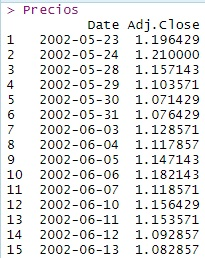
\includegraphics[scale=.75]{Graficos/HeadPrecios.jpg}
   \caption{Datos Log Rendimientos.}
    \label{Datos Log Rendimientos.}
\end{figure}

Algunas de las estadísticas más relevantes son las siguientes: El precio mínimo de cierre registrado fue de 0.37 dólares el 9 de octubre de 2002, mientras que el precio máximo de cierre se registró el 10 de julio de 2020 por un monto de 439.17 dólares. Por otro lado, Netflix presentó un promedio de precios al cierre por 72.82 dólares por acción a lo largo de estos 18 años y mostró una mediana de 14.54 dólares. 
\\\\
Asimismo, con ayuda de los cuantiles, observamos un sesgo a la izquierda, es decir, una simetría positiva que indica, en general, que el precio de cierre de Netflix se mantuvo en constante crecimiento.
\\\\
Finalmente corroboramos, a través del comando class(), que este dataset es del tipo series de tiempo y además su frecuencia o periodicidad es igual a 251.
\newpage
\subsection{Análisis Gráfico.}
A continuación mostramos las gráficas más representativas de nuestra base de datos, e interpretamos una a una, con el fin de tener un mayor conocimientos de nuestros datos antes de intentar ajustar algún modelo.
\begin{figure}[!ht]
    \centering
    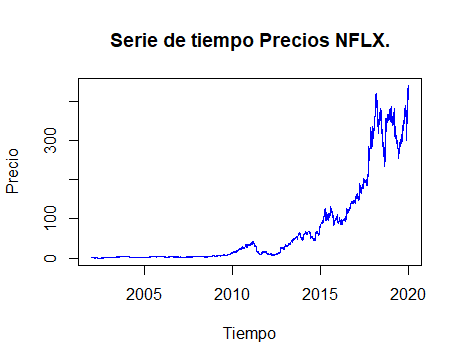
\includegraphics[scale=.75]{Graficos/PreciosNFLT.png}
   \caption{Precios Netflix.}
    \label{Precios Netflix.}
\end{figure}
\\\\

La gráfica anterior muestra los precios de cierre de Netflix, en la cual podemos observar, como bien se mencionaba en la ``Introducción a la Base``, que dichos precios se han visto afectados por diversos sucesos. En particular, se observa que: A partir de 2010 y hasta 2011, comienzan a subir los precios como respuesta al quiebre de Blockbuster y su apertura en América Latina y el Caribe; De manera similar, también se presenta una subida en 2015 a consecuencia de los 17 millones de nuevos usuarios. Finalmente, en 2019 muestra una importante caída como respuesta a una gran disminución en el número de usuarios y fallo de proyecciones de ventas a nivel mundial.   

Por otro lado, se observa en general una varianza creciente, por lo cual proseguiremos a transformar los datos, obteniendo como resultado el siguiente gráfico.

\begin{figure}[!ht]
    \centering
    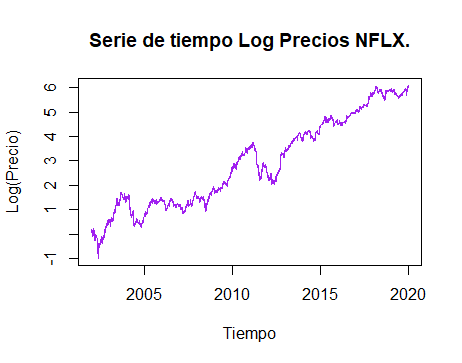
\includegraphics[scale=.70]{Graficos/LOGPRECIOSNFLT.png}
  \caption{Log Precios Netflix.}
    \label{Log Precios Netflix.}
\end{figure}
\newpage
A través de la figura \ref{Log Precios Netflix.} verificamos que nuestra transformación, la cual fue aplicar el logaritmo natural a los precios, resultó correcta, por el hecho de que se muestran un poco más compactos y con menos fluctuaciones.
\\\\
Posteriormente, de acuerdo con la teoría investigada, definimos una nueva transformación como la diferencia entre los precios logarítmicos, la cual nos permitirá trabajar de manera más adecuada, y al resultado lo llamaremos "Log Rendimientos". Como se muestra en la figura \ref{Log Rendimientos.}.

\begin{figure}[!ht]
    \centering
    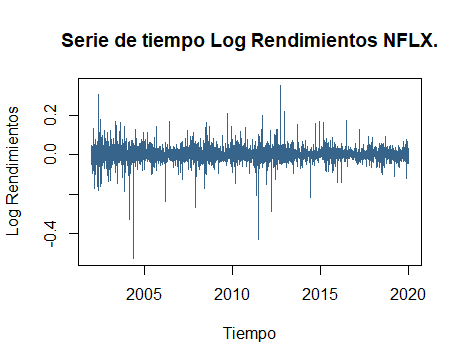
\includegraphics[scale=.7]{Graficos/Rendimientos.png}
  \caption{Log Rendimientos.}
    \label{Log Rendimientos.}
\end{figure}

Este gráfico será analizado con mayor detenimiento en secciones posteriores, pero a grandes rasgos vemos: no tendencia, oscilación alrededor del cero y la variabilidad va cambiando. Además de que muestra dos significativas caídas una antes de 2005 y otra en 2010. Junto con una gran subida entre 2010 y 2015.  
\\\\
\\\\
A continuación se muestran los histogramas de los Precios y los Log Precios de Netflix, con sus respectivas densidades empíricas. 

\begin{figure}[htbp]
    \centering
    \subfigure{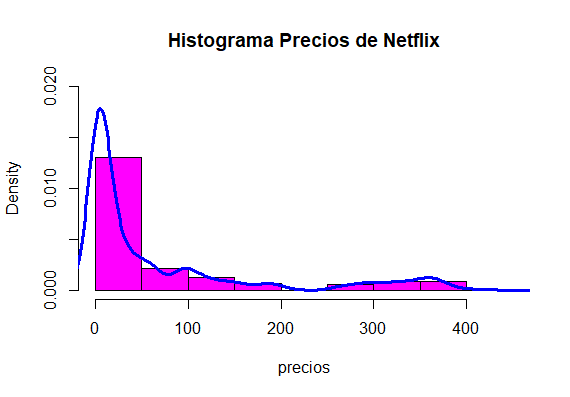
\includegraphics[width=60mm]{Graficos/HIstPreciosNFLX.png}}\vspace{10mm}
    \subfigure{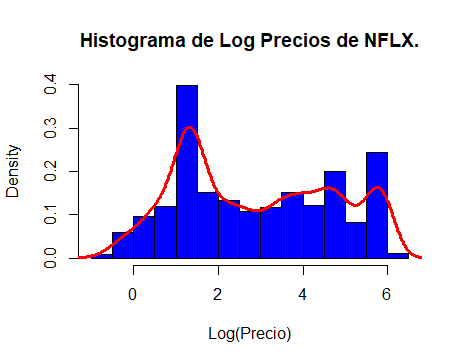
\includegraphics[width=60mm]{Graficos/Hist Log Precios NFLX.png}}
    \caption{Histogramas.} 
    \label{HistogramasPN.}
\end{figure}

Con lo que respecta al gráfico del lado izquierdo, notamos que la mayoría de los datos se concentran entre los 0 y 50 dólares, por lo cual podemos interpretar a los precios que oscilan más allá de los 400 dólares como valores atípicos dentro de nuestra serie de tiempo.
\\\\
Análogamente, el gráfico del lado derecho confirma nuestra interpretación, pues como bien sabemos, el aplicar una transformación logaritmo resulta en un reescalamiento de los datos. Por lo cual, seguimos notando un pico importante entre el 0 y el 2 del Log(Precio). 
\\\\
\newpage
Por último, presentamos el histograma correspondiente con los Log Rendimientos, así como su función de densidad empírica.
\\\\
\begin{figure}[htbp]
    \centering
    \subfigure{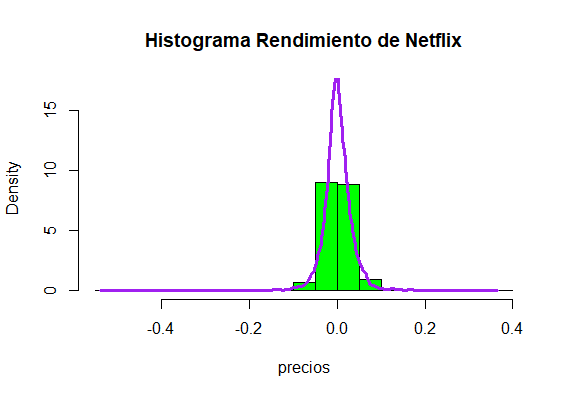
\includegraphics[width=80mm] {Graficos/Hist Log Rendi NFLX.png}}\vspace{10mm}
    \subfigure{
\includegraphics[width=55mm]{Graficos/Kurtosis.png}}
    \caption{Histograma Log Rendimientos} 
    \label{Histogramas Log Rendimientos.}
\end{figure}
\\\\
\\\\
Observemos que en general, se presentan colas muy pesadas, al igual que una kurtosis muy por encima de la que presentaría una distribución normal, estás características nos ayudarán a definir nuestro modelo más adelante.    







\section{Métodos de descomposición}
Ahora observemos las componentes de nuestra serie de tiempo. Cabe mencionar que las características de nuestra serie nos darán como resultado componentes diferentes a las que se acostumbró ver en la modelación ARIMA.
\\\\
Utilizando la función decompose como si se tratara de un modelo aditivo podremos acceder rápidamente a las componentes. A continuación podemos ver nuestra componente de tendencia, que tal y como se esperaba, no se alejó mucho del cero.

\begin{figure}[!ht]
    \centering
    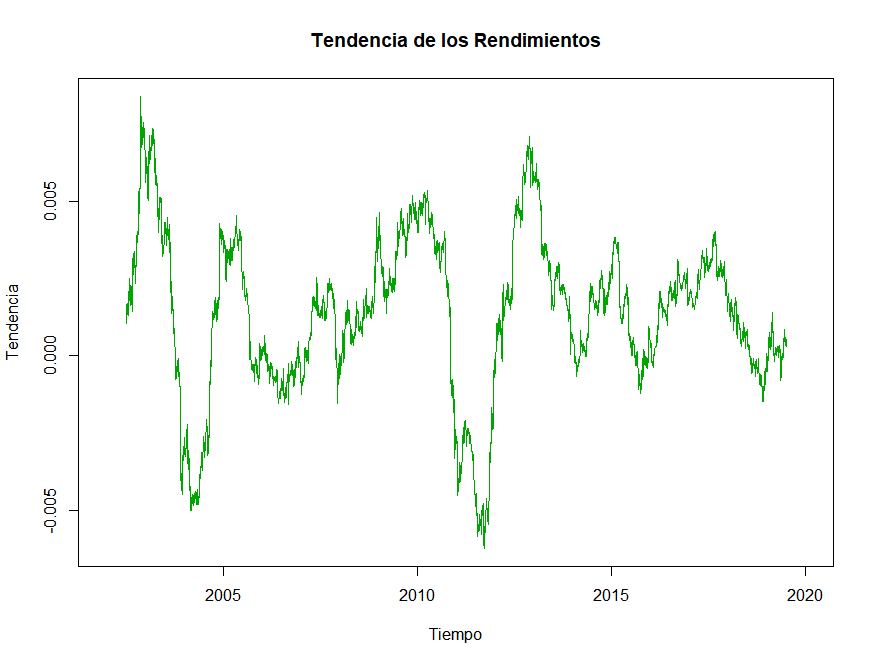
\includegraphics[scale=.35]{Graficos/CompRendimientos.png}
    \caption{Componente de tendencia de los rendimientos}
    \label{comp_tendencia}
\end{figure}

\newpage
La siguiente gráfica a observar será la de nuestra componente de ciclos estacionales. Podemos notar ligeramente que se tratan de ciclos anuales lo cual tiene sentido, al tratarse de rendimientos de acciones a pesar de su alta volatilidad, hay épocas que destacan por la reactivación de la actividad económica a lo largo del año.

\begin{figure}[!ht]
    \centering
    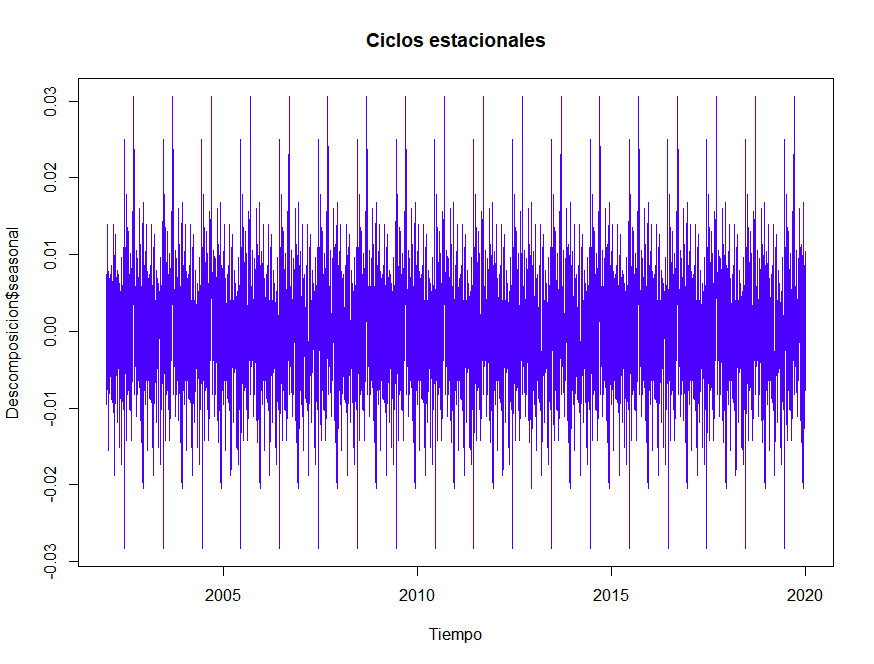
\includegraphics[scale=.35]{Graficos/CompCiclos.png}
    \caption{Componente de tendencia de los ciclos estacionales}
    \label{componente_ciclos}
\end{figure}


Finalmente observemos nuestra componente aleatoria. Trataremos de modelarla tomando en cuenta sus características de alta volatilidad.

\begin{figure}[!ht]
    \centering
    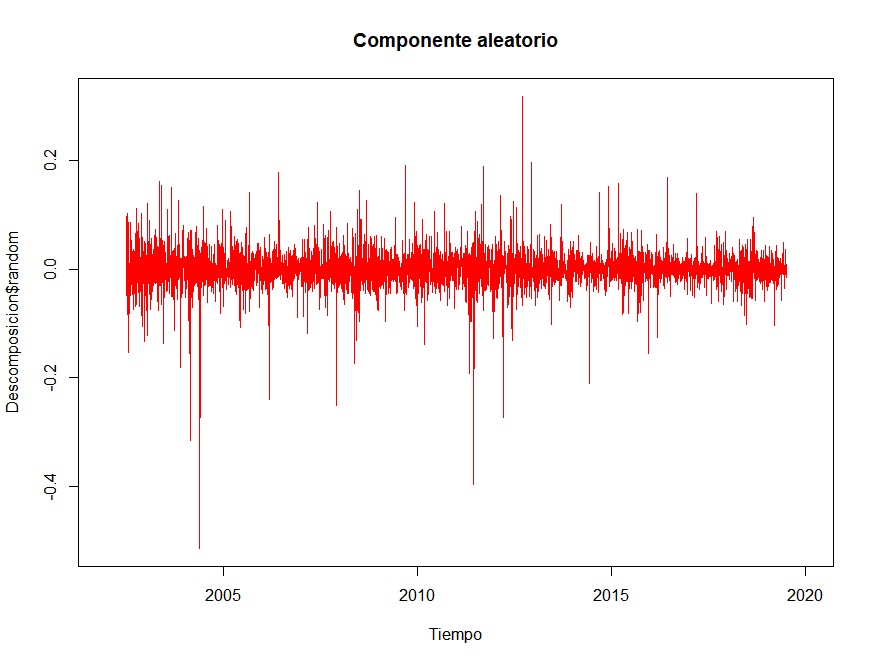
\includegraphics[scale=.33]{Graficos/CompRand.png}
    \caption{Componente aleatoria de los rendimientos}
    \label{componente_aleatoria}
\end{figure}

\newpage


\section{Ajuste serie de Tiempo}
\bigskip
Debido a que la volatilidad varía através del tiempo en  los retornos de Netflix, los modelos clásicos de series de tiempo como los \textit{Arima } o \textit{ARMA} no son adecuados para modelarla, ya que una de las premisas es que la varianza es constante.

\begin{figure}[!ht]
    \centering
    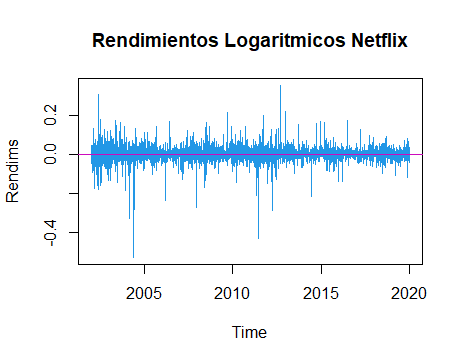
\includegraphics[scale=.75]{Graficos/RendimientosLog.png}
    \caption{Rendimientos Logaritmicos}
    \label{Rendimientos Logaritmicos}
\end{figure}

Notemos que esta serie no tiene tendencia, los valores oscilan alrededor del 0 y además es fácil ver que la variabilidad va cambiando, se presenta períodos largos de alta volatilidad seguidos por períodos de baja volatilidad, lo que indica \textbf{apriori} la presencia de heterocedasticidad. Para comprobar este hecho, miraremos las gráficas de las funciones de auto correlación y auto correlación parcial, tanto de la serie como la del cuadrado de esta, para comprobar que no existe correlación de primer orden, pero si de orden cuadrático. Como se puede comprobar en la gráfica \ref{ACF}.


\begin{figure}[ht]
    \centering
    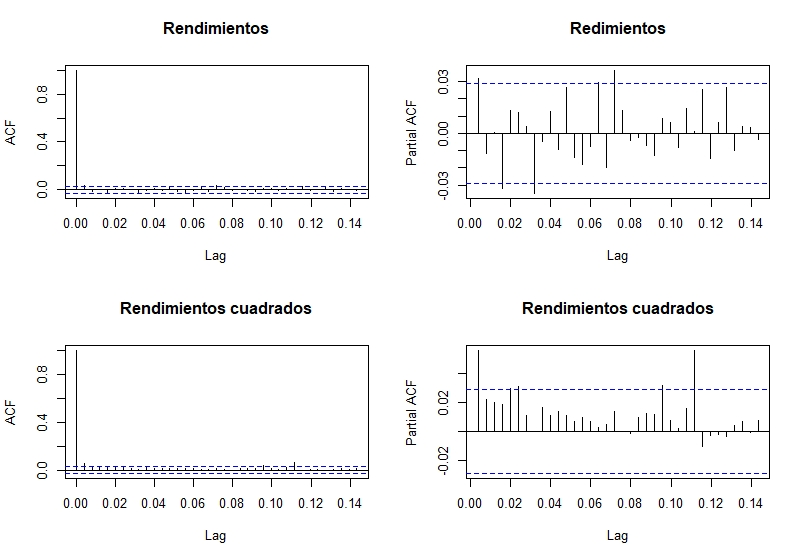
\includegraphics[width=0.75\textwidth]{Graficos/ACFRendi.jpeg}
    \caption{Correlogramas}
    \label{ACF}
\end{figure}


\newpage

Es por ello que se decidió modelar nuestros rendimientos con un \textit{modelo generalizado, auto-regresivo, condicionalmente heterocedástico} que por sus siglas en ingles se denota
\textbf{GARCH(q,p)}
\newline Decimos que es: 

\begin{itemize}
\item Generalizado: Ya que toma en cuenta tanto las observaciones recientes como las históricas.
\item  Autorregresivo: Ya que la variable dependiente se regresa en sí misma.
\item  Condicional: La varianza futura depende de la varianza histórica.
\item Heterocedástico: La varianza cambia en función de las observaciones.
\end{itemize}






En otras palabras, el modelo \textbf{GARCH} encuentra la volatilidad promedio a medio plazo mediante una autorregresión que depende de la suma de los errores retrasados q periodos y de la suma de varianzas retrasadas p periodos. De tal manera que los modelos GARCH(p,q) modelan la volatilidad de la siguiente forma:

\begin{equation}
   \sigma_t^2 =\omega+   \sum^p_{p=1}\alpha_p \epsilon_{t-p}^2 +  \sum^q_{q=1}\beta_q \sigma_{t-q}^2
\end{equation}

Por otro lado, al considerar rendimientos logarítmicos, los modelos GARCH nos permiten observarlos mediante la siguiente expresión:

\begin{equation}
   r_t =\mu_t +  \epsilon_t 
\end{equation}

Donde $\epsilon_t  $ recibe el nombre de innovación y puede ser visto como: 

\begin{equation}
   \epsilon_t =\sigma_t\eta_t 
\end{equation}

Siendo $\eta_t  $ una variable a la cual se le asocia una distribución no necesariamente Normal.
A su vez, como $\epsilon_t$ depende 
$\eta_t$, nuestras innovaciones o residuos tendrán asociada de igual forma una distribución que tendremos que intuir a partir del sesgo y las colas de la distribución de nuestros rendimientos.
\bigskip

Antes de comenzar a proponer nuestros posibles modelos, es conveniente hacer un análisis del histograma de los rendimientos para entender su comportamiento. Se puede apreciar en el gráfico \ref{Histograma de Rendimientos} que se presenta una gran concentración de los datos cerca de la media, es decir, la distribución es leptocúrtica y con colas pesadas. Por otro lado presenta un sesgo en los datos, por lo que podríamos pensar que la distribución de los rendimientos se asemeja a una t-student sesgada.
\begin{figure}[ht]
    \centering
    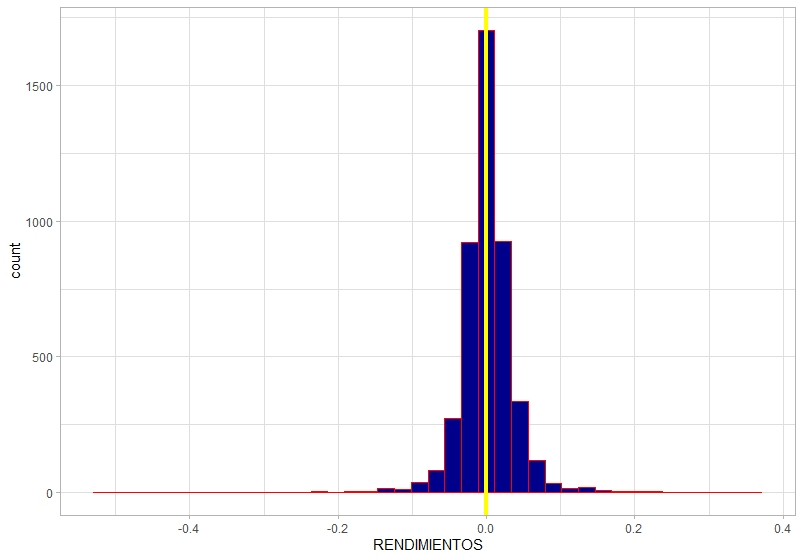
\includegraphics[scale=.5]{Graficos/HistogramaRend.jpeg}
    \caption{Histograma de Rendimientos}
    \label{Histograma de Rendimientos}
\end{figure}

\newpage

Suponiendo dicha distribución, nos dimos a la tarea de probar con distintos modelos GARCH(p,q) suponiendo un modelo autorregresivo de medias móviles para el componente de media observado en la ecuación (2) y modificando los grados de los polinomios de retraso (p y q) asociados a los residuos y a la varianza. 
\bigskip
\smallskip

Nuestro primer criterio para determinar cual es el mejor modelo es encontrar el que tiene el AIC y BIC mas pequeño, pues recordemos que estas pruebas se rigen bajo el principio de parsimonia es decir buscan el modelo mas simple que mejor describa las variables.
\bigskip
En la tabla  \ref{Modelos Propuestos} podemos observar una serie de modelos candidatos que podrian ajustarse a nuestros rendimientos
\input{Tablas/Comparacion de modelo }

Podemos apreciar en la tabla \ref{Modelos Propuestos} que el mejor resulta ser el modelo \textbf{GARCH(1,2)} compuesto con un modelo \textbf{ARMA(1,1)} para el componente de media $\mu_t$, es decir, estamos considerando a los rendimientos de la siguiente forma:

 \begin{equation}
   r_t =  \mu + \phi(r_{t-1} - \mu) + \theta \epsilon_{t-1} +  \epsilon_t
\end{equation}

Donde $\mu$ es una constante a estimar, $\phi$ es el coeficiente del componente autorregresivo AR y $\theta$ es el coeficiente del componente de medias móviles MA.




\section{Supuestos}

Una vez elegido nuestro modelo debemos de comprobar que efectivamente cumple las condiciones bajo las cuales están sustentadas:

\begin{itemize}
    \item Parametros significativos 
    \item Independecia de los residuos
    \item Independecia de los residuos al cuadrado 
    \item La distribucion empirica se distribuye con una t-student sesgada  

\end{itemize}

\bigskip
\subsection{Parametros Significativos}
\bigskip
En la tabla \ref{Caracteristicas del modelo} se muestran los valores estimados de los parámetros, las respectivas desviaciones estándar, y el p-valor correspondiente a las pruebas de hipótesis son 
\bigskip
$$H_0:\theta_i =0 \quad vs.\quad H_1:\theta_i \not= 0$$

\newpage

   Para estos parámetros. La hipótesis $H_{0}$ se rechaza a un nivel de significancia del 5$\%$
   

\begin{table}[htbp]

\begin{center}
    

\begin{tabular}[!h]{|c | c | c | } \hline
	
	\rowcolor{cyan} \multicolumn{3}{ |c| }{ \textbf{Modelo GARCH (1,2)   }} \\ \hline
	 \hline
	

\rowcolor{red}  Parámetro & Valor Estimado & P-value\\\hline
	  
  $\mu$      &	0.001827	& 	0.000024  \\\hline
  $ar_1$     &	-0.985978   & 0.000000   \\\hline
  $ma_1$     &	0.989861    & 	0.000000 \\\hline
  $\omega$   &	0.000018    & 	0.000131 \\\hline
  $\alpha_1$ &	0.053250 	&	0.000000 \\\hline
  $\beta_1$  &	0.120970	&	0.004485 \\\hline
  $\beta_2$  &	0.816019	&	0.000000 \\\hline
    skew     & 1.073804 	&	0.000000 \\\hline
    shape     &	3.153194	&	0.000000 \\\hline
    	     
	
	\end{tabular}

	\label{Caracteristicas del modelo}
	\caption{Caracteristicas del modelo}
\end{center}

\end{table}
 
 Resumiendo, de esta tabla podemos decir que tenemos suficiente información estadística para decir que todos  los parámetros son significativamente distintos de 0. La ecuación de varianza de este modelo resulta ser:
 
 \begin{equation}
   \sigma_t^2 =0.000018+  0.053250  \epsilon_{t-1}^2 + 0.120970  \sigma_{t-1}^2 + 0.120970  \sigma_{t-2}^2
\end{equation}

Y el modelo de los rendimientos es:

 \begin{equation}
   r_t =  0.001827 - 0.985978(r_{t-1} - 0.001827) + 0.989861\epsilon_{t-1} +  \epsilon_t
\end{equation}



 \subsection{Independencia de residuos}
 Para este supuesto se realizó la prueba de hipótesis Ljung-Box cuyas hipótesis son 
 
 \begin{itemize}
  \centering
    \item[$H_{0}$] \textit{: Los residuales se distribuyen de forma independiente } 
    \item [$H_{1}$] \textit{:Los residuales no se distribuyen de forma independiente }
 \end{itemize}
 \bigskip
los resultados de esta prueba se pueden apreciar en la tabla \ref{Ljung-Box Test en Residuos estandarizados}.
\bigskip

\begin{table}[h]
 
\begin{center}
    

\begin{tabular}[!h]{ |c |  c |  } \hline
	
	\rowcolor{cyan} \multicolumn{2}{ |c| }{ \textbf{Ljung-Box Test en Residuos estandarizados }} \\ \hline
	 \hline
	

\rowcolor{red}   Lag & P-value \\\hline
	  
	                1	& 0.07379 \\\hline
                    5	& 0.18209  \\\hline
                    9	& 0.57767   \\\hline
                    
	
	\end{tabular}
      \caption{Ljung-Box Test en Residuos estandarizados}
	\label{Ljung-Box Test en Residuos estandarizados}
	
\end{center}

\end{table}



Como conclusión de esta tabla podemos decir que los residuos estandarizados obtenidos por el modelo no tienen correlación entre sí para los retrasos  1, 5 y 9. 
\\
\newpage
 
Esto se puede apreciar visualmente en la gráfica \ref{ACF Residuales} en la cual se muestra un buen comportamiento de las autocorrelaciones de los residuos estandarizados pues la mayoría de ellas se encuentran comprendidas en las bandas de confianza.


\begin{figure}[h]
    \centering
    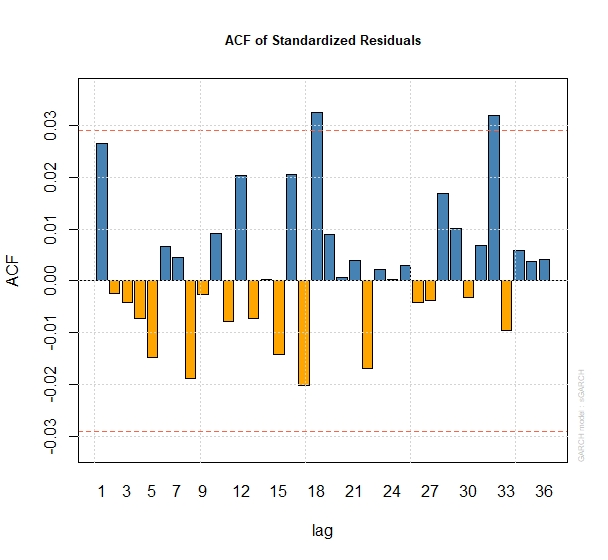
\includegraphics[scale=.4]{Graficos/ACF Residuales sta.jpeg}
    \caption{ACF Residuales}
    \label{ACF Residuales}
\end{figure}

\bigskip
Ahora como se menciono en la implementación del modelo, los modelos \textbf{GARCH}  dependen del cuadrado de los errores retrasados p periodos atrás
es por ello que es importante aplicar la misma prueba de hipótesis a los residuos cuadráticos estandarizados.
\\
Los resultados de esta prueba se pueden ver en la tabla \ref{Ljung-Box Test en Residuos cuadraticos estandarizados}.


\begin{table}[!h]
 
\begin{center}
    

\begin{tabular}[!h]{ |c |  c |  } \hline
	
	\rowcolor{cyan} \multicolumn{2}{ |c| }{ \textbf{Ljung-Box Test en Residuos cuadráticos estandarizados }} \\ \hline
	 \hline
	

\rowcolor{red}   Lag & P-value \\\hline
	  
	                1	& 0.9838 \\\hline
                    8	& 0.9914  \\\hline
                    14	& 0.9980  \\\hline
                    
	
	\end{tabular}

\caption{Ljung-Box Test en Residuos cuadraticos estandarizados}
	\label{Ljung-Box Test en Residuos cuadraticos estandarizados}
	
\end{center}

\end{table}



De esta manera, podemos afirmar que tenemos suficiente información estadística para decir que los residuales cuadráticos estandarizados son independientes, siendo esto confirmado  por la gráfica \ref{ACF cuadraticos}.
\bigskip


\begin{figure}[h]
    \centering
    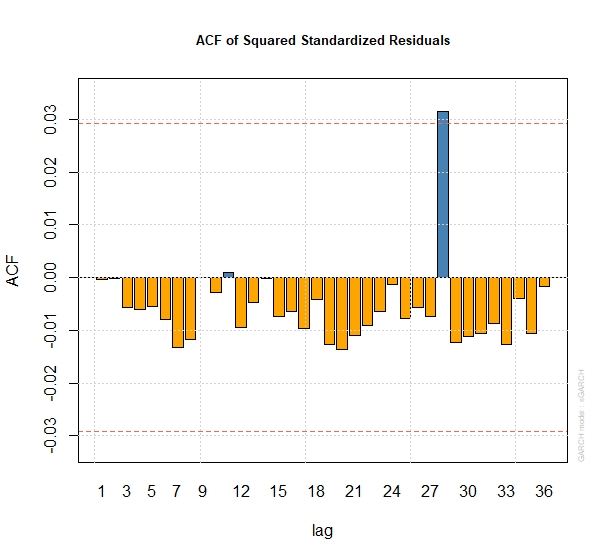
\includegraphics[scale=.5]{Graficos/ACF Residuales.jpeg}
     \caption{ACF Residuales cuadraticos}
    \label{ACF cuadraticos}
\end{figure}




\subsection{Ajuste a ditribucion Empirica}
\bigskip
Para determinar si la distribución propuesta es correcta, en este caso la t-student sesgada, se llevo a cabo una prueba de bondad ajuste, la cual  compara la distribución teórica de los residuos estandarizados con la distribución empírica seleccionada. La hipótesis nula es que la distribución empírica y teórica es idéntica.
\bigskip
\begin{table}[h]

\begin{center}
    

\begin{tabular}[!h]{|c | c | } \hline
	
	\rowcolor{cyan} \multicolumn{2}{ |c| }{ \textbf{Prueba de Bondad de Ajuste de Pearson}} \\ \hline
	 \hline
	

\rowcolor{red}  Group  & P-value\\\hline
	  
  20   	& 	0.1806 \\\hline
  30    &   0.1972 \\\hline
  40    & 	0.1954 \\\hline
  50    & 	0.1024 \\\hline

	
	\end{tabular}

	\label{Person}
	\caption{Prueba de Hipotesis Person}
	
\end{center}

\end{table}


 Notemos que en cualquier caso el p-value$>$ 0.05 por lo que no se rechaza la hipotesis nula, para comprobar esto, podemos observar el qq-plot y el histograma de los residuos.
 
 \begin{figure}[h]
    \centering
    \subfigure{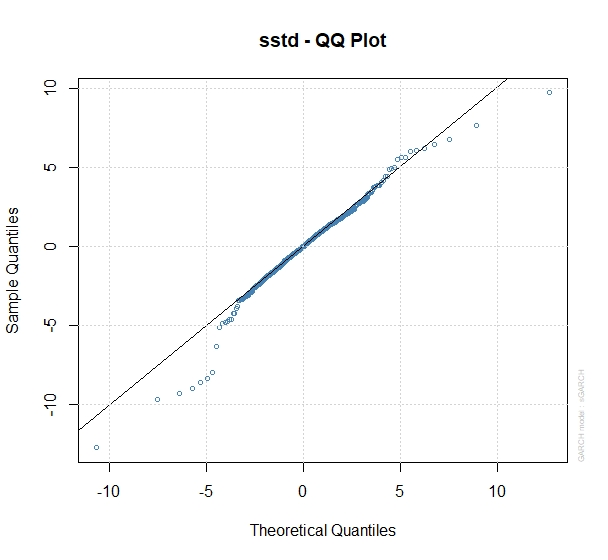
\includegraphics[width=60mm]{Graficos/QQPlotSST.jpeg}}\vspace{10mm}
    \subfigure{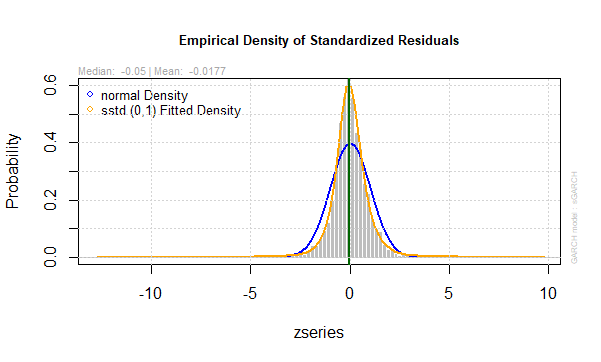
\includegraphics[width=100mm]{Graficos/DensityResiduals.png}}
    \caption{Ajuste a distribucion de t-studet.} 
    \label{Ajuste a distribucion de t-studet.}
\end{figure}
 
 
 
\subsection{Media cero de los residuos}
\bigskip
 Para verificar el supuesto de que los residuos mantienen una media igual a 0 se efectuó la prueba t-Student cuyo p-value nos permite afirmar este hecho. En este caso el p-value resulto de 0.3355 por lo que no se rechaza la hipótesis nula.
 

 Además de ello si hacemos el calculo de la media de los residuo veremos que esta resulta -0.0005258295, un valor muy cercano al 0.
 \newpage
\subsection{Varianza constante de los residuos}

 La  manera  de  comprobar  dicho  supuesto  sobre  el  ruido  blanco  del  modelo  es  mediante  herramientas gráficas.
 
\begin{figure}[!h]
    \centering
    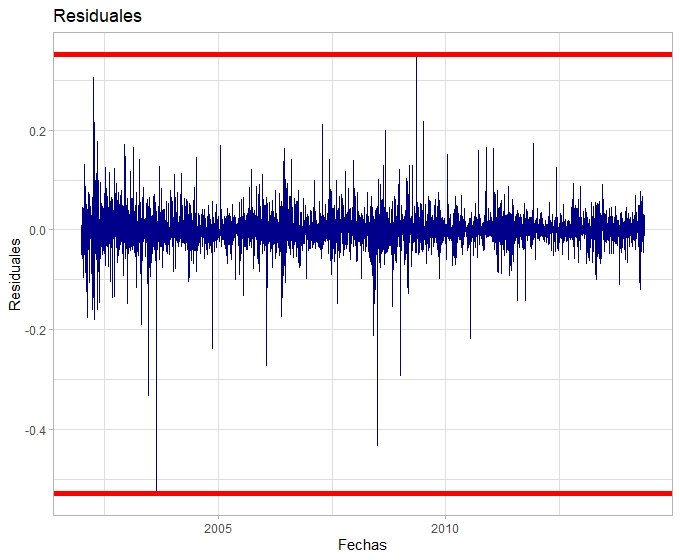
\includegraphics[width=0.55\textwidth]{Graficos/ResidualesApa.jpeg}
      \caption{Residuales}
    \label{Graficas de residuos}
\end{figure}
\bigskip

 
 Como  es  posible  observar,  la  varianza  de  los  residuales  no  es  creciente  pues  se  pueden  encerrar las observaciones entre dos bandas. En nuestro caso las bandas corresponden al valor mínimo y máximo delos residuos, por lo tanto, con total seguridad podemos decir que el supuesto se cumple con  éxito.
 


\section{Pronósticos y Conclusiones}
En general, sabemos que las fluctuaciones cambiarias componen uno de los riesgos más importantes a los que se enfrentan los inversionistas. Por ello es de gran importancia realizar el pronóstico de volatilidad para la toma de decisiones relacionadas con la administración de portafolios. De esta forma, los modelos denominados de heteroscedasticidad condicional autorregresiva nos permiten realizar una buena estimación. 
\\\\
Hsieh (1989) sostiene que en la familia de los modelos ARCH/GARCH no hay uno que se
pueda considerar como el modelo general para pronosticar los diferentes tipos de cambio.
Sin embargo, es conveniente señalar que en particular el uso del modelo GARCH se
justifica porque permite especificaciones más parsimoniosas que el modelo ARCH, sus propiedades son bastante conocidas porque es la especificación más común entre los modelos de la familia ARCH/GARCH y se ajusta muy bien a los datos de variables financieras, principalmente
cuando las observaciones son de alta frecuencia. \footnote{Ortiz-Arango, F., \& Cabrera Llanos, A. (2012). Pronóstico de la volatilidad cambiaria peso-dólar mediante modelos GARCH (pp. 3-5). México.}

 Para un periodo de 20 días, (aproximadamente un més de cotizaciones), hicimos uso de la función \textit{ugarchforecast()} la cual nos permite obtener las bandas de confianza dentro de las cuales se espera que  los rendimientos futuros se encuentren (Figura \ref{pronostico_serie}) y por otro lado, también nos permitió obtener el comportamiento futuro de la varianza de dichos rendimientos. (Figura \ref{pronostico_varianza})
\begin{figure}[!ht]
    \centering
    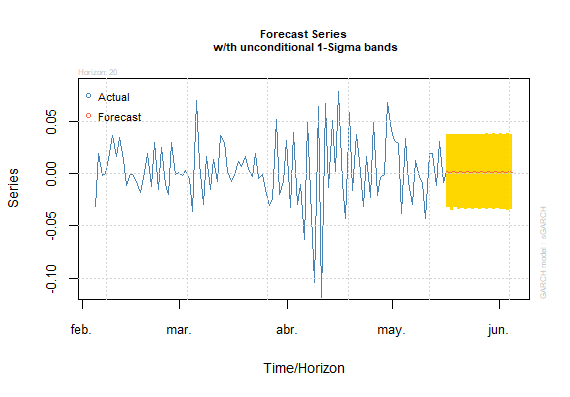
\includegraphics[scale=.8]{Graficos/pronostico_serie_20dias.png}
    \caption{Pronóstico de rendimientos con bandas}
    \label{pronostico_serie}
\end{figure}

\begin{figure}[!ht]
    \centering
    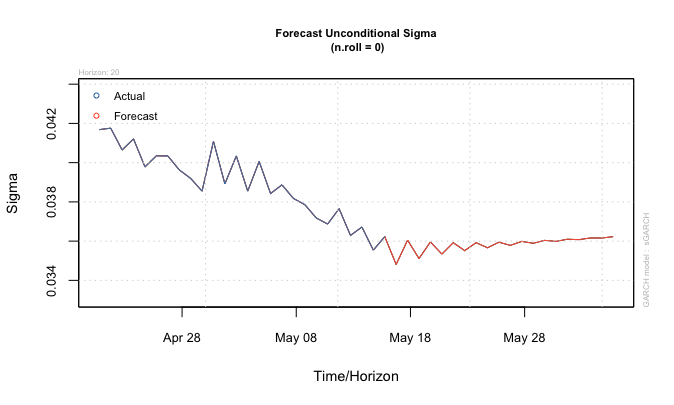
\includegraphics[scale=.5]{Graficos/Pronostico de Varianza.png}
    \caption{Pronóstico de varianza}
    \label{pronostico_varianza}
\end{figure}

\newpage
Recordando que el pronóstico para este tipo de modelos se basa en el valor esperado de las innovaciones y, por lo tanto, en la densidad elegida. Los pronósticos de un paso adelante se basan en el valor de los datos anteriores, mientras que los n pasos adelante (n$>$ 1) se basan en la expectativa incondicional de los modelos. Por esto, las gráficas anteriores muestran datos bajo la volatilidad ``unconditional``. La capacidad de lanzar el pronóstico un paso a la vez se implementa con el argumento \textit{n. Roll}, que controla cuántas veces se debe lanzar el pronóstico n. Adelantado. El argumento predeterminado de \textit{n. Roll = 0} denota que no hay desplazamiento y devuelve el pronóstico n. Anticipado estándar. Fundamentalmente, dado que n. Roll depende de que haya datos disponibles para basar el pronóstico móvil.
\\\\
Como podemos observar de la Figura \ref{pronostico_serie} y la Figura \ref{pronostico_varianza} , aquella que muestra las bandas de confianza de los rendimientos hace evidente que para el siguiente mes se tiene esperado un comportamiento poco volátil, considerando que en periodos anteriores los rendimientos habían fluctuado de manera agresiva. Esto se ve reafirmado por el gráfico de la varianza estimada, pues es claro que tiende a estabilizarse con el tiempo. 




\begin{thebibliography}{X }
\bibitem{Garch}Bauwens, L., Laurent, S., $\&$ Rombouts, J. V. (2006). Multivariate GARCH models: a survey. Journal of applied econometrics, 21(1), 79-109.

\bibitem{Lundbergh} Lundbergh, S., $\&$ Teräsvirta, T. (2002). Evaluating GARCH models. Journal of Econometrics, 110(2), 417-435.

\bibitem{Francq}Francq, C., $\&$ Zakoian, J. M. (2019). GARCH models: structure, statistical inference and financial applications. John Wiley $\&$ Sons.

\bibitem{Silvennoinen}Silvennoinen, A., $\&$ Teräsvirta, T. (2009). Multivariate GARCH models. In Handbook of financial time series (pp. 201-229). Springer, Berlin, Heidelberg.

\bibitem{Teräsvirta}Teräsvirta, T. (2009). An introduction to univariate GARCH models. In Handbook of financial time series (pp. 17-42). Springer, Berlin, Heidelberg.
\bibitem{Engle}Engle, R. (2001). GARCH 101: The use of ARCH/GARCH models in applied econometrics. Journal of economic perspectives, 15(4), 157-168.

\end{thebibliography}
\end{document}
